
\subsection*{1.}

\paragraph{a.} Dans l'énoncé la dernière indication signifie que \(p(R \cap B) = 0{,}36\).

\paragraph{b.}

\begin{center}
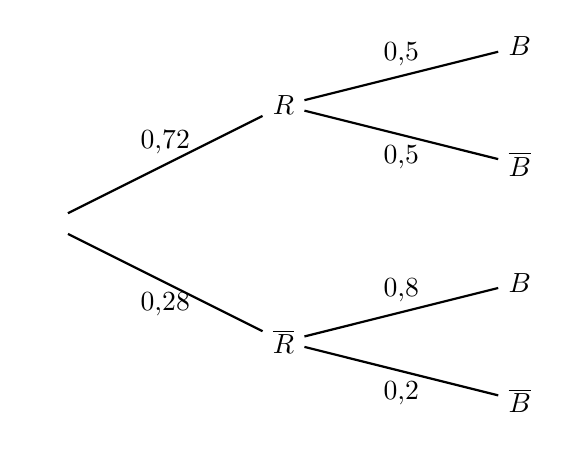
\begin{tikzpicture}[thick, scale=1.5]
\node (P_-1_0) at (-2,-1.5) {$\phantom{A}$};
\node (P_0_0) at (0,-0.5) {$R$};
\draw (P_-1_0) -- (P_0_0) node[midway, above] {$0{,}72$};
\node (P_1_0) at (2,-0) {$B$};
\draw (P_0_0) -- (P_1_0) node[midway, above] {$0{,}5$};
\node (P_1_1) at (2,-1) {$\overline{B}$};
\draw (P_0_0) -- (P_1_1) node[midway, below] {$0{,}5$};
\node (P_0_2) at (0,-2.5) {$\overline{R}$};
\draw (P_-1_0) -- (P_0_2) node[midway, below] {$0{,}28$};
\node (P_1_2) at (2,-2) {$B$};
\draw (P_0_2) -- (P_1_2) node[midway, above] {$0{,}8$};
\node (P_1_3) at (2,-3) {$\overline{B}$};
\draw (P_0_2) -- (P_1_3) node[midway, below] {$0{,}2$};
\end{tikzpicture}
\end{center}

\paragraph{c.} On a :
\[
p(\overline{R} \cap B) = p(\overline{R}) \times p_{\overline{R}}(B) = 0{,}28 \times 0{,}8 = 0{,}224.
\]

D'après la loi des probabilités totales :
\[
p(B) = p(R \cap B) + p(\overline{R} \cap B) = 0{,}36 + 0{,}224 = 0{,}584.
\]

\subsection*{2.}

\paragraph{a.}

\[
\begin{array}{|c|c|c|c|c|}
\hline
x_i & 25{,}50 & 23{,}50 & 11{,}60 & 10{,}50 \\
\hline
p(X = x_i) & 0{,}36 & 0{,}36 & 0{,}224 & 0{,}056 \\
\hline
\end{array}
\]

\paragraph{b.} On a :
\begin{align*}
E(X) &= 0{,}36 \times 25{,}5 + 0{,}36 \times 23{,}5 + 0{,}224 \times 11{,}6 + 0{,}056 \times 10{,}5 \\
&= 20{,}8264 \approx 20{,}83 \text{ €}.
\end{align*}

